\section{Sets, Not Neighbors}
\label{sec:problem}

\paragraph{Evidence-set retrieval.} A memory holds the history $H=(r_1,\dots,r_n)$ of one user, where a round $r_i$ consists of a user turn, the assistant turn that follows it, the images attached to them, and the session date. For a question $q$, the evidence set $G(q)\subseteq H$ contains the rounds on which the answer depends, and a retriever returns a set $S(q)\subseteq H$ from which a reader answers. We score retrieval per question by full-set recall,
\begin{equation}
\fsr(q)=\mathbf{1}\left[\,G(q)\subseteq S(q)\,\right],
\label{eq:fsr}
\end{equation}
together with the number of opened rounds $|S(q)|$, which sets how much the reader must read. Full-set recall is the per-question form of the all-recall measure of multi-hop retrieval~\citep{gutierrez2024hipporag}. Unlike recall@$k$ and coverage, which average over items, it drops to zero when a single member is missing, which is exactly when a count or a comparison fails. The goal of evidence-set retrieval is a small $S(q)$ with $\fsr(q)=1$.

\paragraph{Neighbors suffice for text memory.} With \texttt{gemini-3.8-flash} as the reader, cosine retrieval of raw turns is within one point of the full history on LoCoMo~\citep{maharana2024locomo} (0.781 against 0.790) and LongMemEval-S~\citep{wu2025longmemeval} (0.941 against 0.950), with paired intervals that include zero (Figure~\ref{fig:setsize}a; Appendix~\ref{app:text}).

\paragraph{Multimodal questions ask for sets.} MemEye contains 371 questions over eight long histories with shared images, and removing all visual information lowers full-context accuracy from 0.819 to 0.191, whereas on Mem-Gallery it barely changes (Figure~\ref{fig:setsize}b). Here the same reader falls 0.130 below full context with top-10 retrieval and 0.079 below it with top-40 retrieval, and the gap concentrates on incomplete sets: it is 0.034 when the top 10 rounds contain the complete evidence and 0.296 when they do not. A larger budget only postpones the problem, since completeness decays with the size of the set at every budget, and top-40 retrieval recovers only 0.30 of the sets with six or more rounds (Figure~\ref{fig:setsize}c). Many misses involve aliases defined elsewhere in the history, which a similarity score between the question and one round cannot resolve but a reader of the whole history can.

\begin{figure*}[t]
\centering
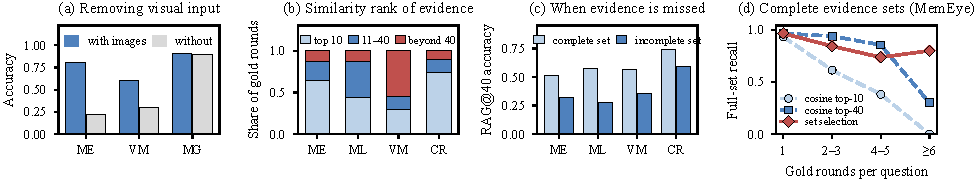
\includegraphics[width=\textwidth]{figures/problem.pdf}
\caption{(a)~Cosine retrieval minus full-context reading (strong reader, paired 95\% intervals). (b)~Accuracy with and without visual input: full context with the strong reader on MemEye and half of Mem-Gallery, annotated evidence with the lightweight reader on VisualMem (chance 0.25). (c)~Full-set recall and (d)~opened rounds on MemEye by the number of gold rounds per question.}
\label{fig:setsize}
\end{figure*}
